% !TEX program = xelatex
\documentclass[a4paper,UTF8]{ctexart}
\usepackage[hyphens]{url}
\usepackage[unicode=true,colorlinks,breaklinks=true,urlcolor=blue,linkcolor=blue,bookmarksnumbered=true]{hyperref}
\usepackage{latexsym,amssymb,amsmath,amsbsy,amsopn,amstext,amsthm,amsxtra,mathrsfs,color,multicol,bm,calc,ifpdf}
\usepackage{graphicx}
\usepackage{diagbox}   % 绘制表格斜线
\usepackage{enumerate}
\usepackage{epstopdf}
\usepackage{fancyhdr}
\usepackage{subfigure}
\usepackage{listings}
\usepackage{multirow}
\usepackage{makeidx}
\usepackage{xcolor} 
\usepackage{fontspec}                            % 建立索引宏包
\graphicspath{{figures/}}  % 设置图片搜索路径
\theoremstyle{plain} \newtheorem{theorem}{定理}[section]
\theoremstyle{plain} \newtheorem{definition}{定义}[section]
\theoremstyle{plain} \newtheorem{lemma}{引理}[section]
\theoremstyle{plain} \newtheorem{proposition}{命题}[section]
\theoremstyle{plain} \newtheorem{example}{例}
\theoremstyle{plain} \newtheorem{remark}{注}
\theoremstyle{plain} \newtheorem{corollary}{推论}[section]
\newfontfamily\courier{Courier New}
\lstset{linewidth=1.1\textwidth,
        numbers=left, %设置行号位置 
        basicstyle=\small\courier,
        numberstyle=\tiny\courier, %设置行号大小  
        keywordstyle=\color{blue}\courier, %设置关键字颜色  
        %identifierstyle=\bf,
        commentstyle=\it\color[cmyk]{1,0,1,0}\courier, %设置注释颜色 
        stringstyle=\it\color[RGB]{128,0,0}\courier,
        %framexleftmargin=10mm,
        frame=single, %设置边框格式  
        backgroundcolor=\color[RGB]{245,245,244},
        %escapeinside=``, %逃逸字符(1左面的键),用于显示中文  
        breaklines, %自动折行  
        extendedchars=false, %解决代码跨页时,章节标题,页眉等汉字不显示的问题  
        xleftmargin=2em,xrightmargin=2em, aboveskip=1em, %设置边距  
        tabsize=4, %设置tab空格数  
        showspaces=false %不显示空格  
        basicstyle=\small\courier
       }  
\def\UrlBreaks{\do\/\do-\do\_\do\a\do\p}    % url 自动换行
% \def\UrlBreaks{\do\A\do\B\do\C\do\D\do\E\do\F\do\G\do\H\do\I\do\J
% \do\K\do\L\do\M\do\N\do\O\do\P\do\Q\do\R\do\S\do\T\do\U\do\V
% \do\W\do\X\do\Y\do\Z\do\[\do\\\do\]\do\^\do\_\do\`\do\a\do\b
% \do\c\do\d\do\e\do\f\do\g\do\h\do\i\do\j\do\k\do\l\do\m\do\n
% \do\o\do\p\do\q\do\r\do\s\do\t\do\u\do\v\do\w\do\x\do\y\do\z
% \do\.\do\@\do\\\do\/\do\!\do\_\do\|\do\;\do\>\do\]\do\)\do\,
% \do\?\do\'\do+\do\=\do\#}   
\newenvironment{mysolution}{{\color{blue} 解}: }{{\color{magenta}\qed}}
\newcommand\diff{\,{\mathrm d}} %定义微分d
\newcommand{\p}[3]{\frac{\partial^{#1}#2}{\partial{#3}^{#1}}}  %定义求偏导算子
\newcommand{\ucite}[1]{\textsuperscript{\cite{#1}}}  %参考文献引用: 上标用\ucite{ }, 文中用\cite{ }

\begin{document}
\title{

\includegraphics[width=0.65\textwidth]{onepiece.pdf}\\
\vspace{2em}
\textbf{SVM 学习笔记}}
\author{\emph{李向阳} \quad {\color{blue}d1142845997@gmail.com}
}
\date{}


\maketitle
\thispagestyle{empty}

\newpage


\tableofcontents

\newpage

\section{引入}
支撑向量机(Support Vector Machine)是一种的分类方法, 当然它也可以用于回归. 不过我们这里主要讨论分类, 仍然主要针对二分类.

在 Logistic 回归模型中, 我们知道决策边界是$\bm{\theta}^{T} \bm{x} = 0$, 一个样本属于正类的概率为
\begin{equation*}
h_{\bm{\theta}}(\bm{x}) = \sigma (\bm{\theta}^{T} \bm{x})
\end{equation*}

一个样本$\bm{x}$归为正类当且仅当$h_{\bm{\theta}}(\bm{x}) \geqslant 0.5$, 或者等价地, 当且仅当$\bm{\theta}^{T} \bm{x} \geqslant 0$, 显然, 给定一个样本$\bm{x}$, $\bm{\theta}^{T} \bm{x}$的值越大, 那么我们就越有信心将其归为正类, 反之, $\bm{\theta}^{T} \bm{x}$的值越小, 那么我们就越有信心将其归为负类, 换句话说, 我们希望所有的样本计算出的$\bm{\theta}^{T} \bm{x}$的值与$0$相差都尽量的大.

SVM的思想与此类似, 我们希望找到一个超平面, 使得样本点到超平面的距离尽量的大. 下面我们就来介绍SVM模型.

为了讨论的方便, 我们这次稍微改换一下记号. 之前在 Logistic 回归中, 我们用类标签$y = 1$表示正类, 用$y = 0$表示负类, 在 SVM 中, 我们改用$y = 1$表示正类, $y = -1$表示负类(只是为了推导的方便). 所谓 SVM 模型, 是用如下公式来刻画: 
\begin{equation*}
y = \mathrm{sign} (f(\bm{x})) = \mathrm{sign}(\bm{w}^{T} \bm{x} + b) 
\end{equation*}

即令$f(\bm{x}) = \bm{w}^{T} \bm{x} + b$, 如果$f(\bm{x}) > 0$, 就令$y = 1$(把样本归为正类), 如果$f(\bm{x}) < 0$, 就令$y = -1$(把样本归为负类).

注意这里与 Logistic 回归中记号的不同, 样本$\bm{x}$有$n$个特征, 即$\bm{x} = (x_{1}, x_{2}, \cdots, x_{n})^{T}$, 参数不再用$\bm{\theta} = (\theta_0, \theta_1, \cdots, \theta_{n})$来表示, 而是把常数项$\theta_0$单独拿出来用$b$表示, 其它参数用$\bm{w} = (w_1, w_2, \cdots, w_{n})^{T}$表示, 因此我们不必再引入特征$x_{0} = 1$. 此外, 我们这里采用机器学习大纲中的第 2 套记号, 即用$\bm{x}_{i}$表示第$i$个具体的样本, 直接理解为具有$n$个分量的向量, 而不是用$\bm{x}^{(i)}$表示第$i$个样本, 然后设样本个数为$N$.

有了模型, 我们就需要估计出模型参数$\bm{w}$和$b$. 这里我们先不采用统计中的观点(前面的线性回归也好、逻辑回归都可以用最大似然估计), 那么采用什么标准来估计参数呢? 下面就正式讨论 SVM 模型.


\section{基本SVM模型}
\subsection{函数间隔和几何间隔}
我们希望样本点到超平面的距离越远越好, 实际上, 结合上面的分析, 我们这里有 2 个标准, 分别是函数间隔(Functional Margin)和几何间隔(Geometric Margin).

Functional Margin 用$\hat{\gamma}$表示, 其定义为
\begin{equation*}
\hat{\gamma}  = y (\bm{w}^{T} \bm{x} + b) = y f(\bm{x})
\end{equation*}

注意到$\bm{w}^{T} \bm{x} + b > 0$时, $y = 1$, 而$\bm{w}^{T} \bm{x} + b < 0$时, $y = -1$, 因此前面乘上$y$可以保证Functional Margin的非负性. 显然, 我们希望对于所有的样本点, 这个值越大越好, 这个可以成为我们的优化目标.

Geometric Margin 用$\tilde{\gamma}$表示, 其定义就直接是样本点$\bm{x}$到超平面$\bm{w}^{T} \bm{x} + b = 0$的距离. 当然, 我们也希望这个值越大越好, 这个也可以作为我们的优化目标.

二者之间有什么关系呢?

对于一个点$\bm{x}$(实际上是用$n$维向量表示), 设其到超平面的投影点为$\bm{x}_{0}$, 我们知道$\bm{w}$是超平面的一个法向量, 设点$\bm{x}$到超平面的距离为$\gamma$, 则有
\begin{equation}\label{pointreprent}
\bm{x} = \bm{x}_{0} + \gamma \frac{\bm{w}}{||\bm{w}||} \quad (\bm{x} - \bm{x}_{0} = \gamma \frac{\bm{w}}{||\bm{w}||})
\end{equation}

注意这里的$\gamma$是带符号的(可正可负), 在这里, 把它乘上对应的类别$y$刚好就是真正的距离$\tilde{\gamma}$.

由于$\bm{x}_{0}$在超平面上, 满足$f(\bm{x}_{0}) = \bm{w}^{T} \bm{x}_{0} + b = 0$, 即有$\bm{w}^{T} \bm{x}_{0} = -b$, 为了利用此条件, 我们将式(\ref{pointreprent})的两边同时乘以$\bm{w}^{T}$, 可得
\begin{equation*}
\bm{w}^{T} \bm{x}  = \bm{w}^{T} \bm{x}_{0} + \gamma \cdot \frac{\bm{w}^{T} \bm{w}}{||\bm{w}||} = -b + \gamma ||\bm{w}||
\end{equation*}

于是有
\begin{equation*}
\gamma = \frac{\bm{w}^{T} \bm{x} + b}{||\bm{w}||} = \frac{f(\bm{x})}{||\bm{w}||}
\end{equation*}

因此可得 Geometrical Margin 为
\begin{equation*}
\tilde{\gamma} = y \gamma  = \frac{y f(\bm{x})}{||\bm{w}||} = \frac{\hat{\gamma}}{||\bm{w}||}
\end{equation*}

也就是说 Geometrical Margin 和 Functional Margin 相差一个$||\bm{w}||$的缩放因子.


\subsection{SVM的优化目标}
上面已经提到, 对一个样本点进行分类, 它的 Margin 值越大, 分类的 Confidence 越高. 假设我们的样本容量为$N$, 我们定义该样本集合的 Margin 为所有这$N$个点的 Margin 值中最小的那个.

于是, 为了使得分类的 Confidence 高, 我们希望所选择的超平面能够最大化这个 Margin 值. 这里我们有两个 Margin 可以选, 不过 Functional Margin 明显是不太适合用来最大化的一个量, 因为在超平面固定以后, 我们可以等比例地缩放$\bm{w}$的长度和$b$的值, 这样可以使得$f(\bm{x}) = \bm{w}^{T} \bm{x} + b$的值任意大, 亦即Functional Margin $\hat{\gamma}$可以在超平面固定的情况下取得任意大, 而Geometrical Margin $\tilde{\gamma}$则没有这个问题, 因为它还除以了$||\bm{w}||$, 所以缩放$\bm{w}$和$b$的时候$\tilde{\gamma}$的值是不会改变的, 它只随着超平面的变动而变化,因此这是一个更适合的Margin. 因此, 我们的优化目标是 Geometrical Margin $\tilde{\gamma}$, 也即为
\begin{equation*}
\max \tilde{\gamma} = \max \frac{\hat{\gamma}}{||\bm{w}||}
\end{equation*}

当然, 还要满足限制条件, 即样本集合的这个 Margin 值是所有$N$个样本点的 Margin 值中最小的那个, 也就等价于
\begin{equation*}
y_{i} (\bm{w}^{T} \bm{x}_{i} + b) = \hat{\gamma}_{i} \geqslant \hat{\gamma} , i = 1,2,\cdots,N
\end{equation*}

观察这个优化模型, 我们发现, 正如前面指出的, 即使在超平面固定的情况下, $\hat{\gamma}$的值还是可以随着$||\bm{w}||$的变化而无限变大. 由于我们的目标是确定超平面, 而对这个最大值具体是多少并不关心(如同最大似然估计一样), 因此我们必须把这个无关的变量固定下来. 固定的方式有两种: 一是固定$||\bm{w}||$; 二是固定$\hat{\gamma}$. 基于方便推导和优化的目的, 我们选择第二种, 不妨令$\hat{\gamma} = 1$, 此时$\tilde{\gamma} = 1 / ||\bm{w}||$, 我们的优化模型变为
\begin{equation*}
\max \frac{1}{||\bm{w}||}, \quad s.t. \quad y_{i} (\bm{w}^{T} \bm{x}_{i} + b) \geqslant 1, i = 1,2,\cdots,N
\end{equation*}

其等价形式为
\begin{equation*}
\max \frac{1}{2} ||\bm{w}||^{2}, \quad s.t. \quad y_{i} (\bm{w}^{T} \bm{x}_{i} + b) \geqslant 1, i = 1,2,\cdots,N
\end{equation*}


这是一个凸优化问题, 而且是一个二次规划(Quadratic Programming)问题, 通过求解这个优化问题, 我们就可以得到最优参数$\bm{w}$和$b$, 从而也就得到了超平面的方程, 一个分类器也就出现了.现在我们先暂时不管这个优化问题的求解, 而先来看看支撑向量.


\subsection{支撑向量}
直观上来看, 必然存在两个与决策超平面平行的超平面, 而且它们到决策超平面的距离必然相等(均为$\tilde{\gamma}$), 否则可以通过调整来增大$\tilde{\gamma}$的值, 也即它们的间隔(gap)为$2 \tilde{\gamma}$, 这两个超平面上肯定都会有样本点存在, 否则我们就可以扩大 gap, 也就是增大$\tilde{\gamma}$的值了, 这些样本点, 我们就称为支撑向量(我们知道, 在$n$维空间中, 一个点和以原点为起点, 该点为终点的向量是等价的).

显然, 由于这些支撑向量刚好在边界上, 因此它们就是取得最优值的地方, 所以它们满足$y(\bm{w}^{T} \bm{x} + b) = 1$(之前令Functional Margin为 1),而对于所有不是支撑向量的点, 也就是在“阵地后方”的点, 都有$y(\bm{w}^{T} \bm{x} + b) > 1$, 事实上, 当最优的决策超平面确定下来之后, 这些后方的点就完全成了“路人”了, 飘来飘去都不会再有任何影响.

当然, 除了从几何直观上, 支撑向量的概念也可以从其优化过程的推导中得到.

回顾我们的优化模型,如下
\begin{equation*}
\max \frac{1}{2} ||\bm{w}||^{2}, \quad s.t. \quad y_{i} (\bm{w}^{T} \bm{x}_{i} + b) \geqslant 1, i = 1,2,\cdots,N
\end{equation*}

虽然已经有很多优化包可以高效的求解二次规划, 比如我们在数值优化方法中学过用有效集方法求解二次规划, 但是SVM这个优化问题结构很特殊, 通过Lagrange对偶形变换到对偶变量(Dual Variable)的优化问题之后, 可以找到一种更加有效的方法来进行求解. 这也是SVM盛行的一大原因, 通常情况下这种方法比直接使用通用的 QP 优化包进行优化要高效得多. 此外, 在推导过程中, 许多有趣的特征也会被揭露出来, 包括刚才提到的支撑向量的问题.

现在我们就来进行推导, 构造 Lagrange 函数
\begin{equation*}
\mathcal{L} (w,b,\bm{\alpha}) = \frac{1}{2} ||\bm{w}||^{2} - \sum_{i=1}^{N} \alpha_{i} \left( y_{i} (\bm{w}^{T} \bm{x}_{i} + b) - 1  \right)
\end{equation*}

其中$\alpha_{i} \geqslant 0, i = 1,2,\cdots,N$为 Lagrange 乘子(Lagrange multiplier).

关于 Lagrange 对偶形及处理方法我们最优化课上也讲的不多, 其一般原理和结论这里也不进行讨论, 只结合我们当前的优化问题进行论述.

令$\partial \mathcal{L} / \partial \bm{w}$ 和 $\partial \mathcal{L} / \partial b$ 等于零, 可得
\begin{align*}
\p{}{\mathcal{L}}{\bm{w}}  & = 0 \Rightarrow \bm{w} = \sum_{i=1}^{N} \alpha_{i} y_{i} \bm{x}_{i} \\ 
\p{}{\mathcal{L}}{b} &  = 0 \Rightarrow \sum_{i=1}^{N} \alpha_{i} y_{i} = 0
\end{align*}

代回到$\mathcal{L}$中可得
\begin{align*}
\mathcal{L}(\bm{w},b,\bm{\alpha}) & = \frac{1}{2} \sum_{i,j=1}^{N} \alpha_{i} \alpha_{j} y_{i} y_{j} \bm{x}_{i}^{T} \bm{x}_{j} - \sum_{i,j=1}^{N} \alpha_{i} \alpha_{j} y_{i} y_{j} \bm{x}_{i}^{T} \bm{x}_{j} - b \sum_{i=1}^{N} \alpha_{i} y_{i} + \sum_{i=1}^{N} \alpha_{i} \\ 
& = \sum_{i=1}^{N} \alpha_{i} - \frac{1}{2} \sum_{i,j=1}^{N} \alpha_{i} \alpha_{j} y_{i} y_{j} \bm{x}_{i}^{T} \bm{x}_{j}
\end{align*}

由此我们得到关于对偶变量$\bm{\alpha} = (\alpha_1,\alpha_2,\cdots,\alpha_{N})^{T}$的对偶优化问题
\begin{align*}
\begin{cases}
\max\limits_{\bm{\alpha}}  \sum\limits_{i=1}^{N} \alpha_{i} - \dfrac{1}{2} \sum\limits_{i,j=1}^{N} \alpha_{i} \alpha_{j} y_{i} y_{j} \bm{x}_{i}^{T} \bm{x}_{j} \\ 
s.t. \quad \alpha_{i} \geqslant 0, i=1,2,\cdots,N \\ 
\qquad \sum\limits_{i=1}^{N} \alpha_{i} y_{i} = 0
\end{cases}
\end{align*}

如前所述, 这个问题有更加高效的优化算法, 不过具体方法在这里先不介绍, 求得$\bm{\alpha}$之后如何得到$\bm{w}$和$b$也暂不介绍(当然, 求得$\bm{\alpha}$后$\bm{w}$自然就算出来了), 先来看看由推导过程所得到的一些结论.

首先, 是关于超平面, 对于一个样本点$\bm{x}$进行分类, 实际上是通过把$\bm{x}$代入到$f(\bm{x}) = \bm{w}^{T} \bm{x} + b$算出结果然后根据其正符号来进行类别划分的. 在推导中我们得到
\begin{equation*}
\bm{w} = \sum_{i=1}^{N} \alpha_{i} y_{i} \bm{x}_{i}
\end{equation*}

因此可得
\begin{align*}
f(\bm{x}) & = \left( \sum_{i=1}^{N} \alpha_{i} y_{i} \bm{x}_{i} \right)^{T} \bm{x} + b \\ 
& = \sum_{i=1}^{N} \alpha_{i} y_{i} \langle \bm{x}_{i}, \bm{x} \rangle + b
\end{align*}

也就是说, 对于新点$\bm{x}$的预测, 只需要计算它与训练数据点的内积即可(本文中的范数均为普通的2-范数,内积为标准欧氏内积). 这一点至关重要, 是之后使用 Kernel 进行非线性推广的基本前提.

此外, 所谓支撑向量的概念也在这里显示了出来. 事实上, 所有不是支撑向量的那些样本点所对应的系数$\alpha_{i}$都是等于零的, 因此对于新点的内积计算实际上只要针对少量的支撑向量而不是所有的训练样本即可.

为什么非支撑向量对应的$\alpha_{i}$等于零呢? 直观上来理解的话, 就是这些“后方”的点——我们前面提到过, 对超平面是没有影响的, 由于分类完全由超平面决定, 所以这些无关的点并不会参与分类问题的计算, 因而也就不会产生任何影响了. 这个结论也可由刚才的推导中得出, 回顾刚才的 Lagrange 函数
\begin{equation*}
\max_{\alpha_{i} \geqslant 0} \mathcal{L} (\bm{w},b,\bm{\alpha}) = \max _{\alpha_{i} \geqslant 0} \frac{1}{2} ||\bm{w}||^{2} - \sum_{i=1}^{N} \alpha_{i} {\color{red}\left( y_{i} (\bm{w}^{T} \bm{x}_{i} + b) - 1 \right)}
\end{equation*}

注意到如果样本点$\bm{x}_{i}$是支撑向量的话, 上式中红颜色的部分是等于 0 的(因为支撑向量的 Functional Margin 等于 1 ), 而对非支撑向量来说, 其 Functional Margin 是大于 1 的, 因此红颜色部分是大于 0 的, 而$\alpha_{i}$又是非负的, 为了满足最大化, 其$\alpha_{i}$必须等于 0 (也就是说求最大值的过程中, $\alpha_{i}$肯定取 0), 这也就是那些非支撑向量的点的悲惨命运了(当然, 从 KKT 条件也可以说明, 可参考周志华的《机器学习》).

至此, 基本的SVM模型就结束了, 但它不能处理非线性的情况, 下面我们就利用核方法把 SVM 推广到非线性的情况.


\section{核方法(Kernel)}
如果数据集不是线性可分的, 或者说决策边界不是一个线性超平面, 那么我们该怎么办呢?

前面已经介绍过线性回归和 Logistic 回归, 它们看上去是线性模型, 但我们知道, 通过映射到高维空间的办法, 其实它们本质上都可以处理非线性的复杂模型. SVM 当然也不例外, 比如对于$\bm{x} = (x_1, x_2)^{T}$, 我们可以将其映射到 2 次完全多项式, 即
\begin{equation*}
\phi(\bm{x}) = (1,x_1,x_2,x_{1}^{2},x_{2}^{2},x_{1}x_{2})^{T}
\end{equation*}

这样,可以假设超平面的方程为
\begin{equation*}
w_{1} x_{1} + w_{2} x_{2} + w_{3} x_{1}^{2} + w_{4} x_{2}^{2} + w_{5} x_1 x_2 + b = 0
\end{equation*}

我们知道这是一个圆锥曲线, 但是, 如果我们令$z_{1}=x_{1},z_{2}=x_{2},z_{3}=x_{1}^{2},z_{4}=x_{2}^{2},z_{5}=x_{1}x_{2}$, 则上面的方程在新的坐标系下可以写作
\begin{equation*}
\sum_{i=1}^{5} w_{i} z_{i} + b = 0
\end{equation*}

这实际上就是$5$维空间中的一个超平面, 也就是说, 如果我们做一个映射$\phi : \mathbb{R}^{2} \mapsto \mathbb{R}^{5}$, 使$\bm{x}$映射为$\bm{z}$, 那么在新的空间中原来的数据就可能变成线性可分的, 从而就又化为了普通的线性SVM, 可以利用之前推导的方法处理. 这就是 Kernel 方法处理非线性问题的基本思想, 可见下图





这样一来, 如同线性回归和 Logistic 回归一样, 好像我们的问题就解决了, 但是 SVM 还稍微不同(毕竟这一节的主题 Kernel 还没出来呢). 回忆一下, 我们最终得到的分类函数是这样的:
\begin{equation*}
f(\bm{x}) = \sum_{i=1}^{N} \alpha_{i} y_{i} \langle \bm{x}_{i}, \bm{x} \rangle + b
\end{equation*}

现在则是映射后的空间, 即
\begin{equation*}
f(\bm{x}) = \sum_{i=1}^{N} \alpha_{i} y_{i} \langle \phi(\bm{x}_{i}, \phi(\bm{x})) \rangle + b
\end{equation*}

而其中的$\bm{\alpha}$也是通过求解如下对偶问题而得到的
$$
\begin{cases}
\max\limits_{\bm{\alpha}}  \sum\limits_{i=1}^{N} \alpha_{i} - \dfrac{1}{2} \sum\limits_{i,j=1}^{N} \alpha_{i} \alpha_{j} y_{i} y_{j}  \langle \phi(\bm{x}_{i}, \phi(\bm{x})) \rangle \\ 
s.t. \quad \alpha_{i} \geqslant 0, i=1,2,\cdots,N \\ 
\qquad \sum\limits_{i=1}^{N} \alpha_{i} y_{i} = 0
\end{cases}
$$

看似计算并没有什么问题, 但这样实际计算量是非常大的, 刚才我们对一个二维空间做映射,选择的新空间是原始空间的所有一阶和二阶的组合, 得到了5个维度; 如果原始空间是三维, 那么我们会得到 19 维的新空间, 这个数目是爆炸性增长的, 也就给$\phi(\cdot)$的计算带来了非常的困难, 而且如果遇到无穷维的情况(确实会遇到的), 就根本无从计算了. 所以就要轮到 Kernel 出场了.

还是以开始的二维例子进行说明, 对于两个样本$\bm{x}_{1} = (\eta_1, \eta_2)^{T}$和$\bm{x}_{2} = (\xi_1, \xi_2)^{T}$, 设$\phi(\cdot)$是上面的 5 维空间的映射, 即有
\begin{align*}
\phi(\bm{x}_{1}) & = (\eta_1,\eta_2,\eta_{1}^{2},\eta_{2}^{2},\eta_1 \eta_2)^{T} \\ 
\phi(\bm{x}_{2}) & = (\xi_1,\xi_2,\xi_{1}^{2},\xi_{2}^{2},\xi_1 \xi_2)^{T}
\end{align*}

因此映射后要计算的内积为
\begin{equation}\label{mapprod}
\langle \phi(\bm{x}_1), \phi(\bm{x}_2) \rangle  = \eta_1 \xi_1 + \eta_{1}^{2} \xi_{1}^{2} + \eta_{2} \xi_{2} + \eta_{2}^{2} \xi_{2}^{2} + \eta_{1} \eta_{2} \xi_{1} \xi_{2}
\end{equation}

此外, 我们注意到(先别不要管这个是怎么猜到的)
\begin{equation}\label{mapkernel}
\begin{split}
\left(\langle \bm{x}_1, \bm{x}_2 \rangle + 1\right)^{2} & = (\eta_1 \xi_1 + \eta_2 \xi_2 + 1)^{2} \\ 
& = 2 \eta_1 \xi_1 + \eta_{1}^{2} \xi_{1}^{2} + 2 \eta_{2} \xi_{2} + \eta_{2}^{2} \xi_{2}^{2} + 2 \eta_{1} \eta_{2} \xi_{1} \xi_{2} + 1
\end{split}
\end{equation}

二者有很多相似的地方, 实际上, 我们只要把式(\ref{mapprod})某几个维度线性缩放一下, 然后再加上一个常数维度就可以得到式(\ref{mapkernel}), 更具体的, 对于一个样本$\bm{x} = (x_{1},x_{2})^{T}$, 如果我们构造一个这样的映射(与$\phi(\cdot)$类似)
\begin{equation*}
\varphi (\bm{x}) = (\sqrt{2} x_{1}, \sqrt{2} x_{2}, x_{1}^{2}, x_{2}^{2}, \sqrt{2} x_{1} x_{2}, 1)^{T}
\end{equation*}

那么在此映射下, 则有
\begin{equation}\label{newmap}
\langle \varphi(\bm{x}_1), \varphi(\bm{x}_2) \rangle = 2 \eta_1 \xi_1 + \eta_{1}^{2} \xi_{1}^{2} + 2 \eta_{2} \xi_{2} + \eta_{2}^{2} \xi_{2}^{2} + 2 \eta_{1} \eta_{2} \xi_{1} \xi_{2} + 1
\end{equation}

这也就和式(\ref{mapkernel})的结果一模一样了.

区别在什么地方呢?实际上, 式(\ref{newmap})是先映射到高维空间中, 然后再根据内积的公式进行计算; 而式(\ref{mapkernel})则是直接在原来的低维空间中进行计算, 而不需要显式地写出映射后的结果. 回忆刚才提到的映射的维度爆炸, 在前一种方法已经无法计算的情况下, 后一种方法却依旧能从容处理, 甚至是无穷维度的情况也没有问题.

因此, 式(\ref{mapkernel})是非常巧妙的, 本来我们要把原数据通过映射$\varphi(\cdot)$映射到高维空间中进行计算, 但是借助式(\ref{mapkernel})计算可以得到相同的结果, 我们把式(\ref{mapkernel})等式左边的函数就叫做核函数(Kernel Function), 也即
\begin{equation*}
\kappa (\bm{x}_1,\bm{x}_2) = \left(\langle \bm{x}_1, \bm{x}_2 \rangle + 1 \right)^{2}
\end{equation*}

核函数能简化映射空间中的内积运算, 而“碰巧”的是, 在 SVM 模型中, 需要计算的地方数据向量总是以内积的形式出现的. 对比刚才我们写出来的式子, 现在我们的分类函数为
\begin{equation*}
f(\bm{x}) = \sum_{i=1}^{N} \alpha_{i} y_{i} {\color{red}\kappa (\bm{x}_{i},\bm{x})} + b
\end{equation*}

其中$\bm{\alpha}$由如下对偶问题计算而得
$$
\begin{cases}
\max\limits_{\bm{\alpha}}  \sum\limits_{i=1}^{N} \alpha_{i} - \dfrac{1}{2} \sum\limits_{i,j=1}^{N} \alpha_{i} \alpha_{j} y_{i} y_{j}  {\color{red}\kappa (\bm{x}_{i},\bm{x}) } \\ 
s.t. \quad \alpha_{i} \geqslant 0, i = 1,2,\cdots,N \\ 
\qquad \sum\limits_{i=1}^{N} \alpha_{i} y_{i} = 0
\end{cases}
$$

这样一来计算问题就解决了, 避开了直接在高维空间中进行计算, 而结果却是等价的. 但是,因为我们刚才的例子比较简单, 所以可能容易构造出对应于映射$\varphi(\cdot)$的核函数出来, 但是对于任意一个映射, 应该如何构造出对应的核函数呢?

最理想的情况下, 我们希望知道数据的具体形状和分布, 从而可以猜出一个刚好将数据映射成线性可分的$\varphi(\cdot)$, 然后通过这个$\varphi(\cdot)$得出对应的核函数$\kappa(\cdot,\cdot)$, 然后再进行计算即可. 第一步可能还比较容易, 画出数据的分布图, 我们有可能凭肉眼猜到大致的映射. 可是第二步通常是非常困难甚至是完全无法做到的. 不过, 其实第一步也很难做到, 因为二维(也就是有两个特征)还容易画出来, 可是到高维情形呢? 所以, 我们通常并不是精确的寻找这个映射的, 而是先“随便”猜的, 当然可以多猜几次. 既然映射是猜的, 那我们也根本没有必要精确的找出对应于映射的那个核函数, 而且由于它们之间是对应关系, 因此我们干脆直接猜核函数即可. 因为猜一个核函数, 就相当于猜一个映射(虽然不太容易求出来, 也就是说我们并不知道这个映射具体是什么). 由于我们的计算只要利用核函数即可, 所以我们并不关心也没有必要求出所对应的映射的具体形式. 这是利用核函数的关键思想.

当然, 虽说是猜, 但也是有一定讲究的, 因为并不是任意的函数都可以作为核函数. 通常人们会从一些常用的核函数族中选择(根据问题和数据的不同, 选择不同的参数, 实际上就是得到了不同的核函数). 常用的核函数族有
\begin{enumerate}
\item 多项式核
\begin{equation*}
\kappa(\bm{x}_{1},\bm{x}_{2}) = \left( \langle \bm{x}_1,\bm{x}_2 \rangle + R \right)^{d}
\end{equation*}

显然我们刚才举的例子就是这里多项式核的一个特例($R = 1, d = 2$). 虽然比较麻烦, 而且没有必要, 不过这个核所对应的映射实际上是可以写出来的, 新空间的维数是$\mathrm{C}_{n+d}^{d}$, 其中$n$是原始空间的维数.

\item 高斯核
\begin{equation*}
\kappa (\bm{x}_{1},\bm{x}_{2}) = \exp \left( - \frac{||\bm{x}_1 - \bm{x}_2||^2}{2 \sigma^2} \right)
\end{equation*}

这个核就是最开始提到过的会将原始空间映射为无穷维空间的那个家伙. 不过, 如果$\sigma$选的很大的话, 高次特征上的权重实际上衰减的非常快, 所以实际上(数值上近似一下)相当于一个低维的空间; 反过来, 如果$\sigma$选的很小, 则可以将任意的数据映射为线性可分的(这里不给出证明). 当然, 这并不一定是件好事, 也许你已经猜到了, 对, 其随之而来的可能是非常严重的过拟合问题. 不过, 总的来说, 通过调控参数$\sigma$, 高斯核实际上具有相当高的灵活性, 也是使用最广泛的核函数之一. 

在 R 语言和 Python 的实现中, 一般采用如下形式, 并称之为 RBF(Gaussian Radial Basis Function)核
\begin{equation*}
\kappa (\bm{x}_{1},\bm{x}_{2}) = \exp (- \gamma ||\bm{x}_1 - \bm{x}_2||^2)
\end{equation*}

相应的, 也有 Laplace Radial Basis Function (RBF)核, 如下
\begin{equation*}
\kappa (\bm{x}_{1},\bm{x}_{2}) = \exp (- \gamma ||\bm{x}_1 - \bm{x}_2||)
\end{equation*}

\item 线性核
\begin{equation*}
\kappa (\bm{x}_{1},\bm{x}_{2}) = \langle \bm{x}_1,\bm{x}_2 \rangle
\end{equation*}

这实际上就是原始空间中的内积. 这个核存在的主要目的是使得“映射后空间中的问题”和“映射前空间中的问题”两者在形式上统一起来了.

\end{enumerate}

最后, 总结一下: 对于非线性的情况, SVM 的处理方法是选择一个核函数$\kappa(\cdot,\cdot)$, 通过将数据映射到高维空间来解决在原始空间中线性不可分的问题. 由于核函数的优良品质, 这样的非线性扩展在计算量上并没有比原来复杂多少, 这一点是非常难得的. 当然, 这要归功于核方法, 事实上, 除了 SVM 之外, 任何将计算表示为数据点的内积的方法, 都可以使用核方法进行非线性扩展.


\section{软间隔与正则化}
在最开始讨论支持向量机的时候, 我们就假定数据是线性可分的, 亦即我们可以找到一个可行的超平面将数据完全分开. 后来为了处理非线性数据, 使用 Kernel 方法对原来的线性 SVM 进行了推广, 使得非线性的的情况也能处理. 虽然通过映射$\varphi(\cdot)$将原始数据映射到高维空间之后, 能够线性分隔的概率大大增加, 但是对于某些情况还是很难处理. 例如可能并不是因为数据本身是非线性结构的, 而只是因为数据有噪音. 对于这种偏离正常位置很远的数据点, 我们称之为异常值(Outliers), 在我们原来的 SVM 模型里, Outlier 的存在有可能造成很大的影响, 因为超平面本身就是只有少数几个 Support Vector 组成的, 如果这些 Support Vector 里又存在 Outlier 的话,其影响就很大了. 例如下图
\begin{figure}[!htb]
	\centering
	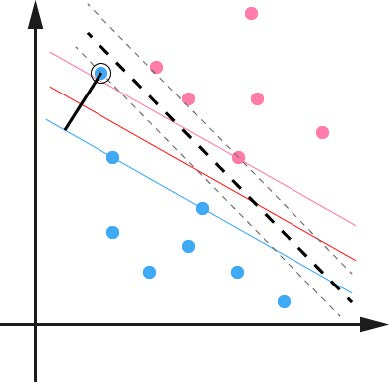
\includegraphics[width=0.85\textwidth]{outlier.jpg}
	\caption{异常值}
	\label{outlier}
\end{figure}

用黑圈圈起来的那个蓝点是一个 Outlier, 它偏离了自己原本所应该在的那个半空间, 如果直接忽略掉它的话, 原来的分隔超平面还是挺好的, 但是由于这个 Outlier 的出现, 导致分隔超平面不得不被挤歪了, 变成图\ref{outlier}中黑色虚线所示(这只是一个示意图, 并没有严格计算精确坐标), 同时 Margin 也相应变小了. 当然, 更严重的情况是, 如果这个 Outlier 再往右上移动一些距离的话, 我们将无法构造出能将数据分开的超平面来.

为了处理这种情况, SVM 允许数据点在一定程度上偏离一下超平面. 例如上图\ref{outlier}中, 黑色实线所对应的距离就是该 Outlier 偏离的距离, 如果把它移动回来, 就刚好落在原来的超平面上, 而不会使得超平面发生变形了. 具体来说, 原来的约束条件
\begin{equation*}
y_{i} (\bm{w}^{T} \bm{x}_{i} + b) \geqslant 1, i = 1,2,\cdots,N
\end{equation*}

现在变成
\begin{equation*}
y_{i} (\bm{w}^{T} \bm{x}_{i} + b) \geqslant 1 - {\color{red}\xi_{i}}, i = 1,2,\cdots,N
\end{equation*}

其中$\xi_{i} \geqslant 0$称为松弛变量(Slack Variable), 对应数据点$\bm{x}_{i}$允许偏离的 Functional Margin 的量. 原来的间隔称为“硬间隔”, 现在的间隔称为“软间隔”. 当然, 如果我们允许$\xi_{i}$任意大的话, 那任意的超平面都是符合条件的了. 所以, 我们要对$\xi_{i}$施加惩罚, 即在原来的目标函数后面加上一项, 使得这些$\xi_{i}$的总和也要最小
\begin{equation*}
\min \frac{1}{2} ||\bm{w}||^2 + {\color{red}C \sum_{i=1}^{N} \xi_{i}}
\end{equation*}

其中$C$是一个参数, 用于控制目标函数中两项(“寻找 Margin 最大的超平面”和“保证数据点偏差量最小”)之间的权重. 注意, 其中$\bm{\xi}$是需要优化的变量(之一), 而$C$是一个事先确定好的常量. 完整地写出来是这个样子
$$
\begin{cases}
\min & \dfrac{1}{2} ||\bm{w}||^2 + C \sum_{i=1}^{N} \xi_{i} \\ 
s.t. & y_{i} (\bm{w}^{T} \bm{x}_{i} + b) \geqslant 1 - \xi_{i} \\ 
\quad & \xi_{i} \geqslant 0, i = 1,2,\cdots,N
\end{cases}
$$

采用 Lagrange 方法, 即构造
\begin{equation*}
\mathcal{L}(\bm{w},b,\bm{\xi},\bm{\alpha},\bm{r})  = \frac{1}{2} ||\bm{w}||^2 + C \sum_{i=1}^{N} \xi_{i} - \sum_{i=1}^{N} \alpha_{i} (y_{i}(\bm{w}^{T} \bm{x}_{i} + b) - 1 + \xi_{i}) - \sum_{i=1}^{N} r_{i}\xi_{i}
\end{equation*}

然后求偏导
\begin{align*}
\p{}{\mathcal{L}}{\bm{w}} & = 0 \Rightarrow \bm{w} = \sum_{i=1}^{N} \alpha_{i} y_{i} \bm{x}_{i} \\ 
\p{}{\mathcal{L}}{b} & = 0 \Rightarrow \sum_{i=1}^{N} \alpha_{i} y_{i} = 0 \\ 
\p{}{\mathcal{L}}{\xi_i} & = 0 \Rightarrow C - \alpha_i - r_i = 0 , i=1,2,\cdots,N 
\end{align*}

将$\bm{w}$代回$\mathcal{L}$并化简, 得到和原来一样的目标函数
\begin{equation*}
\max \sum_{i=1}^{N} \alpha_{i} - \frac{1}{2} \sum_{i,j=1}^{N} \alpha_{i} \alpha_{j} y_{i} y_{j} \langle \bm{x}_{i}, \bm{x}_{j} \rangle
\end{equation*}

不过, 由于我们得到$C - \alpha_{i} - r_{i} = 0$, 而又有$r_{i} \geqslant 0$(作为 Lagrange Multiplier 的条件), 因此有$\alpha_{i} \leqslant C$, 所以整个对偶问题现在写作
$$
\begin{cases}
\max & \sum\limits_{i=1}^{N} \alpha_{i} - \dfrac{1}{2} \sum\limits_{i,j=1}^{N} \alpha_{i} \alpha_{j} y_{i} y_{j} \langle \bm{x}_{i}, \bm{x}_{j} \rangle \\ 
s.t. & 0 \leqslant \alpha_{i} \leqslant C ,i = 1,2,\cdots,N \\ 
\quad & \sum\limits_{i=1}^{N} \alpha_{i} y_{i} = 0
\end{cases}
$$

和之前的结果对比一下, 可以看到唯一的区别就是现在 Dual Variable $\bm{\alpha}$多了一个上限$C$. 而 Kernel 化的非线性形式也是一样的, 只要把$\langle \bm{x}_i,\bm{x}_j \rangle$换成$\kappa (\bm{x}_i,\bm{x}_j)$即可. 这样一来,一个完整的, 可以处理线性和非线性并能容忍噪音和 Outliers 的支持向量机才终于介绍完毕了. Python 的机器学习包 sklearn 中关于 SVM 的模型就是这个, 具体可见\url{http://scikit-learn.org/stable/modules/svm.html}.



\section{SMO 方法}
这里介绍一下对偶问题的数值解法. 前面提到过, 对偶问题有着高效的解法, 其实就是所谓的 Sequential Minimal Optimization (SMO) 方法.

先回忆一下我们之前得出的要求解的对偶问题:
$$
\begin{cases}
\max & \sum\limits_{i=1}^{N} \alpha_{i} - \dfrac{1}{2} \sum\limits_{i,j=1}^{N} \alpha_{i} \alpha_{j} y_{i} y_{j} \kappa (\bm{x}_{i}, \bm{x}_{j} ) \\ 
s.t. & 0 \leqslant \alpha_{i} \leqslant C ,i = 1,2,\cdots,N \\ 
\quad & \sum\limits_{i=1}^{N} \alpha_{i} y_{i} = 0
\end{cases}
$$

对于变量$\bm{\alpha}$来说, 这是一个二次函数. 对于优化问题, 我们最常用的可能就是梯度下降法(这里是求最大值, 不过加个负号就化为最小了), 也就是 Gradient Descent, 其实还有一种叫做 Coordinate Descent 的变种, 它每次只选择一个维度, 例如本模型的$\bm{\alpha} = (\alpha_1,\alpha_2,\cdots,\alpha_N)^{T}$, 它每次选取一个$\alpha_{i}$为变量, 而将$\alpha_1,\cdots,\alpha_{i-1},\alpha_{i+1},\cdots,\alpha_{N}$都看成是常量, 从而原始的问题在这一步变成一个一元函数, 然后针对这个一元函数求最小值, 如此反复轮换不同的维度进行迭代. 这样也确实能求得问题的最小点, 至于原因这里不做介绍. Coordinate Descend 的主要用处在于那些原本很复杂, 但是如果只限制在一维的情况下则变得很简单甚至可以直接求极值的情况, 例如我们这里的问题, 暂且不管约束条件, 如果只看目标函数的话, 当$\alpha$只有一个分量是变量的时候, 这就是一个普通的一元二次函数的极值问题, 是比较容易的.

然而这里还有一个问题就是约束条件的存在, 其实如果没有约束条件的话, 本身就是一个一元二次函数的问题, 极易求解. 但是有了约束条件, 结果就让 Coordinate Descent 失效了, 为什么呢? 比如我们假设$\alpha_1$是变量, 而$\alpha_2,\cdots,\alpha_N$是固定的值的话, 那么其实没有什么好优化的, 直接根据第二个约束条件$\sum\limits_{i=1}^{N} \alpha_{i} y_{i} = 0$, $\alpha_1$的值立即就定下来了, 所以优化无从谈起. 如果还是迭代每个坐标维度, 会发现优化根本无法进行, 因为迭代了一轮之后会发现没有任何进展, 一切都停留在初始值.

所以 Sequential Minimal Optimization (SMO) 就出场了. 它一次选取两个坐标维度来进行优化, 不失一般性, 比如选取$\alpha_1$和$\alpha_2$为变量, 其余为常量, 则根据约束条件我们有
\begin{equation*}
\sum_{i=1}^{N} \alpha_{i} y_{i} = 0 \Rightarrow \alpha_2 = \frac{1}{y_2} \left( - \sum_{i=3}^{N} \alpha_{i} - \alpha_1 y_1 \right) \triangleq y_2 (K - \alpha_1 y_1)
\end{equation*}

其中那个从$3$到$N$的求和加负号视为常量, 所以记为了$K$, 而且由于$y \in \{-1,+1\}$, 所以$y_2$和$1 / y_2$相等, 所以可以变到分子上来.

现在把这个式子代入到原来的目标函数中, 就可以消去$\alpha_2$, 从而可以变成一个一元二次函数, 具体展开的形式这里就不写了, 总之现在变成了一个非常简单的问题——带区间约束的一元二次函数极值问题. 唯一需要注意的就是这里的约束条件, 一个是$\alpha_{1}$本身要满足$0 \leqslant \alpha_{1} \leqslant C$, 另一个就是$\alpha_{2}$也要满足相同的约束条件, 即
\begin{equation*}
0 \leqslant y_2 (K - \alpha_1 y_1) \leqslant C
\end{equation*}

这也是$\alpha_{1}$的约束条件, 同$[0,C]$取交集才是最终的可行区间. 几何直观上看, 原本关于$\alpha_{1}$和$\alpha_{2}$的区间约束构成下图\ref{region}中的绿色的正方形, 而另一个约束条件$\alpha_{1} y_{1} + \alpha_{2} y_{2} = K$实际上是一条直线, 两个集合的交集即是图中红颜色的线段, 投影到$\alpha_1$轴上所对应的区间即为$\alpha_1$的取值范围, 在这个区间内求二次函数的最大值即可完成 SMO 的一步迭代.
\begin{figure}[!htb]
	\centering
	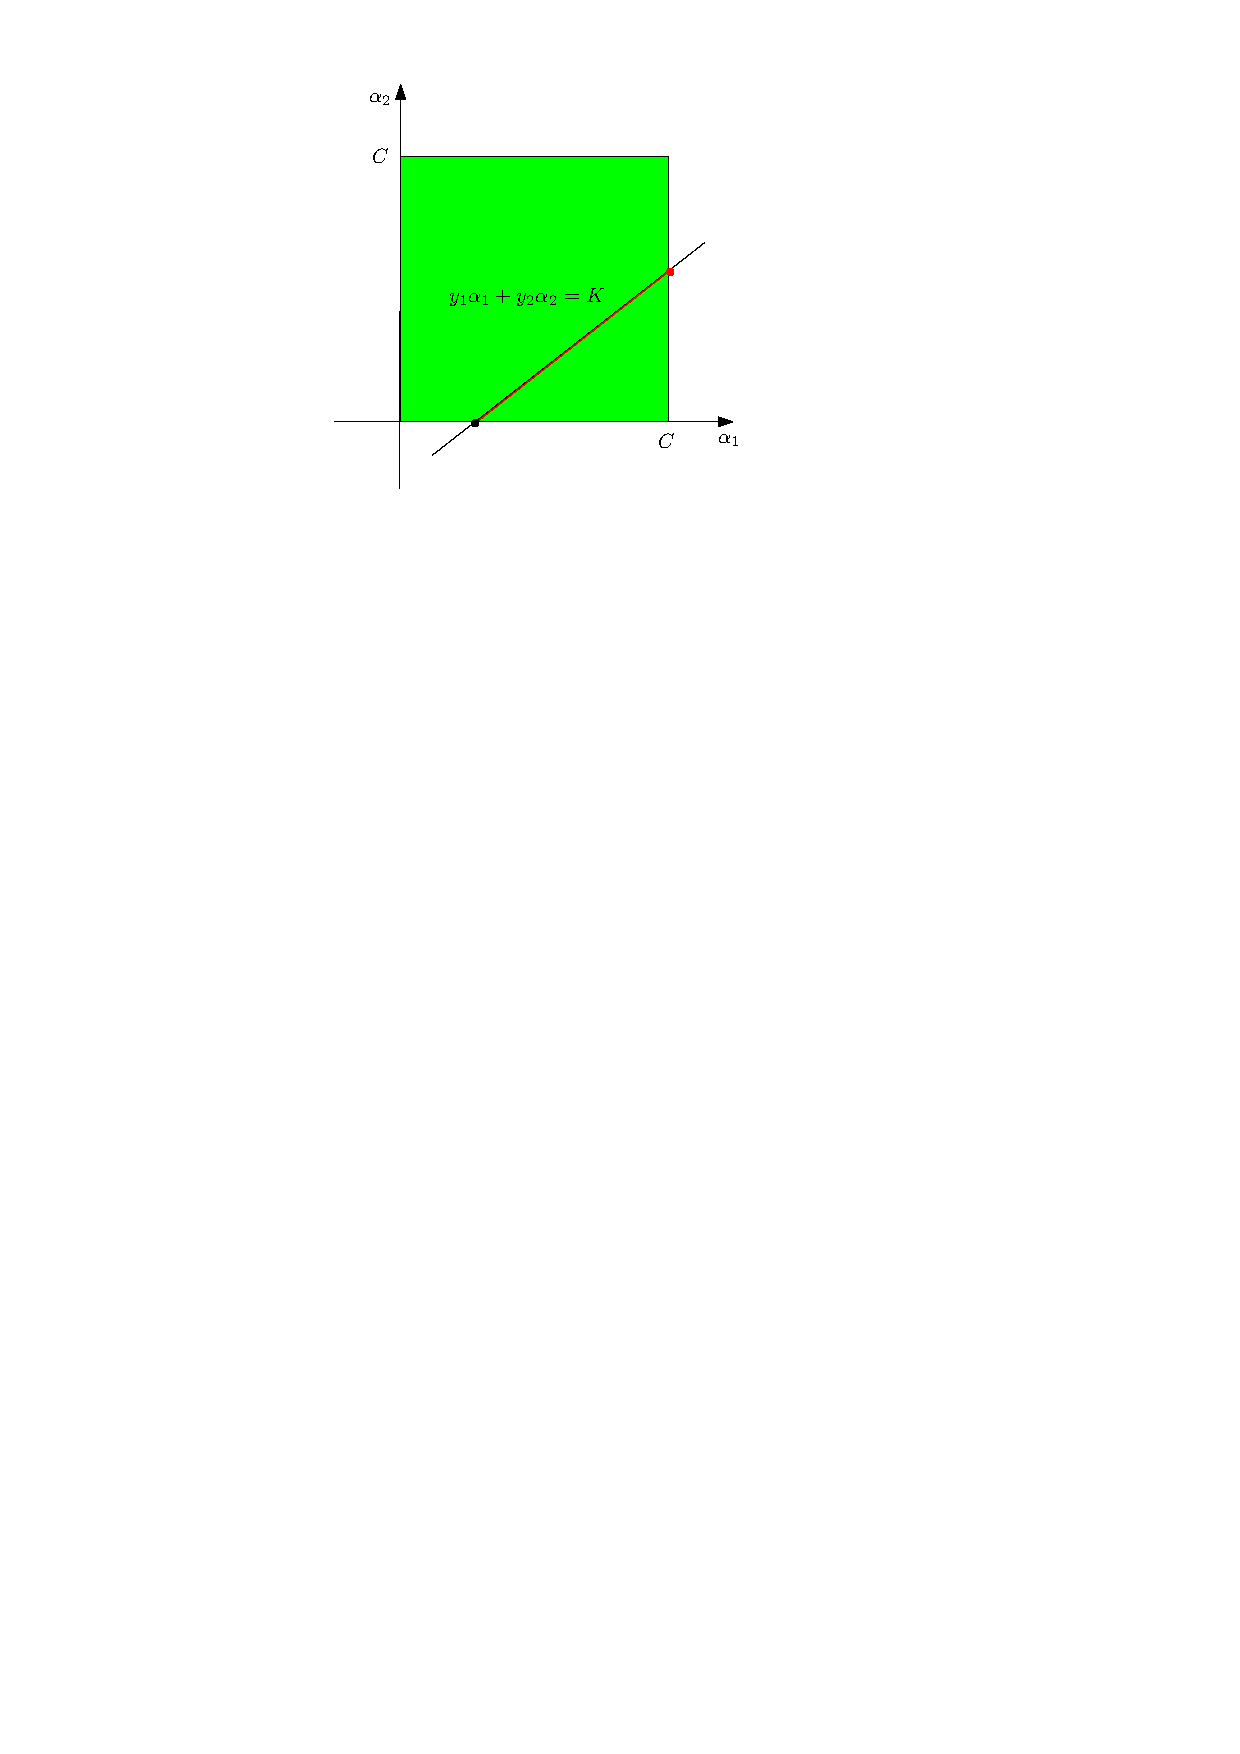
\includegraphics[width=0.85\textwidth]{quader.pdf}
	\caption{可行域示意图}
	\label{region}
\end{figure}

SMO 每次选取不同的两个 Coordinate 维度进行优化, 而且从上面可以看出每一个迭代步骤实际上是一个可以直接求解的一元二次函数极值问题, 所以求解非常高效. 此外, SMO 也并不是依次或者随机地选取两个坐标维度, 而是有一些启发式的策略来选取最优的两个坐标维度, 具体的选取方法(和其他的一些细节)这里就不多说了.

最后, 有一点需要指出的是, 虽然我们从对偶问题的推导中得出了许多 SVM 的优良性质, 但是 SVM 的数值优化(即使是非线性的版本)其实并不一定需要转化为对偶问题来完成, 也有人研究了直接求解原始优化问题的方法, 这里不再多述.



\section{总结}
\subsection{关于 SVM 的补充}
本篇笔记主要参考的是 pluskid 的博客, 难免有些疏漏, 这里提一些补充. 

第一点, 是关于 SVM 的损失函数. 

我们从软间隔说起. 软间隔允许某些样本不满足约束
\begin{equation*}
y_i (\bm{w}^T \bm{x}_i + b) \geqslant 1
\end{equation*}

当然, 在最大化软间隔的同时, 不满足约束的样本应尽可能少. 于是, 优化目标可写为
\begin{equation*}
\min_{\bm{w}, b} \frac{1}{2} ||\bm{w}||^2 + C \sum_{i=1}^{N} \ell_{0 / 1} (y_i (\bm{w}^T \bm{x}_i + b) - 1)
\end{equation*}

其中$C > 0$是一个常数, 也就是正则化参数, $\ell_{0 / 1}$是“0/1 损失函数”
$$
\ell_{0 / 1}(z) = 
\begin{cases}
1, & \mathrm{if} ~ z < 0 \\ 
0, & \mathrm{otherwise}
\end{cases}
$$

显然, 当$C$无穷大时, 优化目标会迫使所有样本均满足硬间隔条件, 与硬间隔的 SVM 等价; 当$C$取有限值时, 优化目标允许一些样本不满足硬间隔约束.

然而, $\ell_{0 / 1}$非凸、非连续, 数学上不好求解, 于是人们通常用其他一些函数来代替$\ell_{0 / 1}$, 称为“替代损失”(surrogate loss). 替代损失函数一般数学性质较好, 如它们通常是凸的连续函数且是$\ell_{0 / 1}$的上界, 比如
\begin{enumerate}[(1)]
\item hinge 损失: $\ell_{\mathrm{hinge}}(z) = \max (0, 1 - z)$

\item 指数损失(exponential loss): $\ell_{\mathrm{exp}}(z) = \exp (-z)$

\item 对数损失(logistic loss): $\ell_{\mathrm{log}} = \log (1 + \exp (-z))$

\end{enumerate}

若采用 hinge 损失, 则优化目标变为
\begin{equation*}
\min_{\bm{w}, b} \frac{1}{2} ||\bm{w}||^2 + C \sum_{i=1}^{N} \max (0, 1 - y_i (\bm{w}^T \bm{x}_i + b))
\end{equation*}

引入松弛变量$\xi_{i} \geqslant 0$, 则可将上式重写为
\begin{align*}
& \min_{\bm{w}, b, \xi_i} \frac{1}{2} ||\bm{w}||^2 + C \sum_{i=1}^{N} \xi_i \\ 
s.t. \quad & y_{i} (\bm{w}^{T} \bm{x}_{i} + b) \geqslant 1 - \xi_{i} \\ 
\quad & \xi_{i} \geqslant 0, i = 1,2,\cdots,N
\end{align*}

这也就是上面的软间隔的 SVM, 不过这次是直接从 hinge 损失函数的角度推出来的.

那么, 能否用其他损失函数替代呢?

当然是可以的. 特别的, 如果我们用对数损失函数代替, 则优化目标变为了
\begin{equation*}
\min_{\bm{w}, b} \frac{1}{2} ||\bm{w}||^2 + C \sum_{i=1}^{N} \log \left( 1 + \exp (- y_i f(\bm{x}_i)) \right)
\end{equation*}

其中$f(\bm{x}_i) = \bm{w}^{T} \bm{x}_i + b$.

回忆一下, 这其实不正是正则化的 Logistic 回归的损失函数吗?

在 Logistic 回归中, 如果用$y = \pm 1$区分正负类, 正则化的损失函数为
\begin{equation*}
J(\bm{\theta}) = \frac{1}{N} \sum_{i=1}^{N} \log (1 + \exp (- y_i f(\bm{x}_i))) + \lambda ||\bm{\theta}||^2
\end{equation*}

因此, 如果用对数损失函数代替, 就变成了 Logistic 回归. 进一步, 如果也引入核函数, 那么可以得到 Kernel Logistic Regression(KLR), 相关讨论这里不再多述. 总之, 替换成一般的损失函数, 我们可以得到一般的模型形式
\begin{equation*}
\min_{f} \Omega(f) + C \sum_{i=1}^{N} \ell (f(\bm{x}_i), y_i)
\end{equation*}

其中$f$表示我们的模型.

第二点, 是关于 SVM 模型的表达方式.

追本溯源, SVM 的基础模型是
\begin{equation*}
f(\bm{x}) = \bm{w}^T \bm{x} + b
\end{equation*}

之后, 引入映射$\phi$后的完整模型为
\begin{equation*}
f(\bm{x}) = \bm{w}^T \phi(\bm{x}) + b
\end{equation*}

而且, 最后我们发现$f(\bm{x})$可以求解表示为
\begin{align*}
f(\bm{x}) & = \bm{w}^T \phi(\bm{x}) + b \\ 
& = \sum_{i=1}^{N} \alpha_i y_i \phi(\bm{x}_i)^T \phi(\bm{x}) + b \\ 
& = \sum_{i=1}^{N} \alpha_i y_i \kappa (\bm{x}, \bm{x}_i) + b
\end{align*}

也就是模型可以通过训练样本的核函数展开, 或者说模型可表示为核函数$\kappa(\bm{x}, \bm{x}_i)$的线性组合. 因此, 有的资料上直接把 SVM 模型表示为
\begin{equation*}
f(\bm{x}; \bm{w}) = \sum_{i=1}^{N} w_i \kappa(\bm{x}, \bm{x}_i) + w_0 
\end{equation*}

其中$w_0, w_1, \cdots, w_N$为模型参数.





\subsection{参考资料}
\begin{enumerate}[(1)]
\item 周志华的《机器学习》

\item pluskid 的系列博客: \url{http://blog.pluskid.org/?page_id=683}, 这是 pluskid 写的支持向量机系列, 写的真是很好, 不多说了, 我的这篇笔记可以当做他博客的一个重新排版吧. 不过还是有一些 SVM 的算法细节(比如 SMO 算法)没有涉及, 当然, 我也没有涉及.

\item zouxy09 的系列博客: \url{http://blog.csdn.net/zouxy09/article/details/17292011}, 写的也不错, 还有自己的 Python 实现. 他博客最后给出的参考资料中也有很多不错.

\item JerryLead 的系列博客: \url{http://www.cnblogs.com/jerrylead/archive/2011/03/13/1982639.html}, 推导比较详细.

\item 博客: \url{http://tullo.ch/articles/svm-py/}, 主要是 Python 代码的实现, 里面二次优化用到了 Python 的 cvxopt 包, 并没有使用 SMO 算法, 与此相似的还有这个: \url{https://gist.github.com/mblondel/586753}, 其对应的博客在 \url{http://www.mblondel.org/journal/2010/09/19/support-vector-machines-in-python/}

\item Andrew Ng 的 Notes 还有他公开课的材料, 其实前面的线性回归和 Logistic 回归他的公开课里都有, 也都参考过, 习题代码均是用 Matlab 所写, 参考代码可见 \url{https://github.com/emilmont/Artificial-Intelligence-and-Machine-Learning/tree/master/ML}

\item 笔记: \url{https://rstudio-pubs-static.s3.amazonaws.com/65566_a44a67a726284943b8f1ec986bf9642d.html}, 用 R 的 e1071 包做 SVM , 感觉是用 RMarkdown 写的, 还有另一篇也不错: \url{https://lagunita.stanford.edu/c4x/HumanitiesScience/StatLearning/asset/ch9.html}

\item stackoverflow: \url{http://stackoverflow.com/questions/22294241/plotting-a-decision-boundary-separating-2-classes-using-matplotlibs-pyplot}, 用 python 的 sklearn 包做了 SVM, 里面有数据的生成和决策边界的画图.

\end{enumerate}



\subsection{SVM的应用场景}





\subsection{SVM的优缺点}




\newpage

\section*{附录}










\end{document}